\documentclass[12pt]{article}
\usepackage[french]{babel}
\usepackage[T1]{fontenc}
\usepackage{listings}
\usepackage{amsmath,amsthm,amssymb,amsfonts}
\usepackage[dvipsnames]{xcolor}
\usepackage{pgfpages}
\usepackage{fullpage}
\usepackage[unicode,psdextra]{hyperref}
\usepackage{graphics}
\usepackage{float}
\usepackage{fancyvrb}

%---------------------------------------%
%             Paramétrage               %
%---------------------------------------%

\lstloadlanguages{C, Caml, Python, SQL}
\lstdefinestyle{CustomCodeBlock}{
    backgroundcolor = \color{gray!10!white},   
    commentstyle = \color{OliveGreen},
    identifierstyle=\color{Tan},
    keywordstyle = \color{MidnightBlue},
    numberstyle = \tiny \color{Gray},
    stringstyle = \color{Orchid},
    basicstyle = \ttfamily \footnotesize,
    breakatwhitespace = false,         
    breaklines = false,                 
    captionpos = b,                    
    keepspaces = false,                 
    numbers = left,                    
    numbersep = 5pt,                  
    showspaces = false,                
    showstringspaces = false,
    showtabs = false,                  
    tabsize = 3,
}
\lstset{style = CustomCodeBlock}



\hypersetup{
	colorlinks,
	citecolor=black,
	filecolor=black,
	linkcolor=black,
	urlcolor=black
}

%---------------------------------------%
%         Information  Générale         %
%---------------------------------------%

\title{Rapport de projet\\ Platformer}
\author{\small FARGEAT Alexis, MAGNIN Mathis, VERDIER Vincent}

%---------------------------------------%
%                Document               %
%---------------------------------------%

\begin{document}

	\maketitle

	\begin{figure}[H]
		\centering
		\begin{BVerbatim}
 _____  ______                               
|  __ \|  ____|                             
| |__) | |__ ___  _ __ _ __ ___   ___ _ __   
|  ___/|  __/ _ \| '__| '_ ` _ \ / _ | '__|
| |    | | | (_) | |  | | | | | |  __| |     
|_|    |_|  \___/|_|  |_| |_| |_|\___|_|   


		\end{BVerbatim}
	\end{figure}

	\tableofcontents
	\newpage

	\section{Introduction}
	
		\begin{center}
			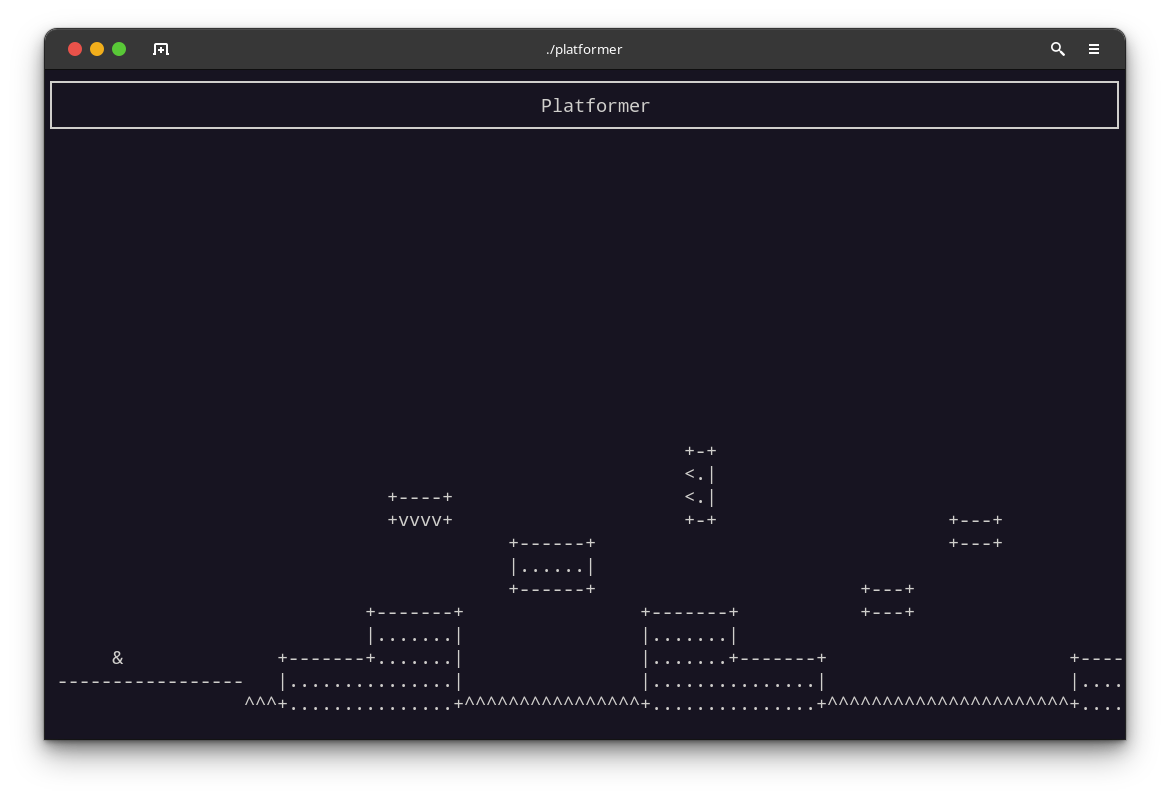
\includegraphics[width = 1\textwidth]{content/image.png}
		\end{center}
	
		Platformer est un jeu de plateforme, où le but est d'arriver au bout d'une carte après de multiple obstacles.
		Ce jeu se rapproche de Mario Bros ou de Geometrydash.
	
		Le jeu est programmé en \textbf{C} et s'utilise dans une console (similaire a MS-DOS).\\

		Le jeu est séparé en 4 grandes parties :
		\begin{itemize}
			\item map : Gestion du chargement et de la création de la carte
			\item affichage : Gestion de l'affichage et des différents menus et du jeu
			\item gameplay : Gestion du mouvement, des collisions, \dots
			\item moteur : Gestion des calculs internes\\
		\end{itemize}
	
	\newpage

	\section{Problèmes rencontrés}

		\subsection{Chargement de la carte}
		
			Au cours de la création du jeu, il a fallu choisir une manière de stocker les données de la carte du jeu.\\


			Nous cherchions une solution permettant un accès simple par les autres parties du programme comme l’affichage.
		
			Nous voulions également avoir la possibilité de modifier la carte du jeu de manière visuelle et sans recompiler le jeu.\\


			Cela nous a amené à choisir de stocker la carte dans un fichier texte qui sera chargé dans le jeu sous forme 
			d’un tableau à deux dimensions de taille dynamique.\\
		
			Au lancement du jeu, les données du fichier texte sont lues et la taille du tableau à allouer est calculée en 
			comptant le nombre de caractères de la ligne du haut de la carte.\\
		
			On stocke alors dans une structure  :
			\begin{itemize}
				\item Les dimensions \((x, y)\) de la carte
				\item Un tableau contenant les données du fichier texte
				\item Un autre tableau utile pour les collisions dont le fonctionnement est détaillé dans la partie Collisions.
			\end{itemize}
		
			Un tableau en \(2D\) de taille dynamique nécessite de libérer la mémoire occupée celui-ci l’arrêt du programme.
		
			Un tableau en \(2D\) peut être vu comme un tableau en \(1D\) stockant des pointeurs qui pointent le premier élément 
			de chaque colonne. Ce tableau en \(1D\) correspond à la première ligne du tableau en \(2D\).
		
			Pour libérer la mémoire occupée par le tableau on libère d’abord la mémoire occupée par chaque colonne puis 
			on libère la mémoire occupée par la première ligne.
			
		\newpage
		
	
		\subsection{Physique et mouvement}
		
		Le mouvement du joueur est modélisé grâce aux équations horaires du mouvement en physique. On applique différentes forces : 
		\begin{enumerate}
			\item Le poids, qui s'applique sur l'axe \(y\)
			\item Les frottements, uniquement sur l'axe des \(x\). Cependant il sont simplifié par une accélération constante dans le sens inverse du mouvement (ils ne sont pas liés à la vitesse du joueur).
		\end{enumerate}
		
		\subsubsection{Sous-structures nécessaire pour l'implémentation}
		
		Cependant, pour il faut d'abord créer un moyen de compter le temps : le compter en secondes directement aurait été compliqué et peu précis, nous avons donc intégrer un compteur d'image qui est incrémenté à chaque passage dans la boucle principale.
		
		\medskip
		
		Ainsi, pour faciliter les modifications de valeurs, on utilise deux structure : \textit{vecteur} et \textit{coords}.
		Ces structures sont composés de deux variable \(x\) et \(y\)(qui décomposent le mouvement sur les deux axes), en flottant pour \textit{vecteur} et entier pour \textit{coords}. Ces deux types ont été nécessaire car lors d'un mouvement les coordonnées changent de très peu, ce qui ne pourrait pas être stocké convenablement dans des entiers, et la position du joueur ne peut être que entière.  
		
		Un autre type, \textit{mouvement} est utilisé pour stocker les actions en cours sur le joueur. La solution retenue ici à été de créer une variable de mouvement pour la vitesse et l'accélération mais en décomposant le mouvement en \(x\) et \(y\). Cette structure mouvement contient une valeur flottante, mais également une horloge, qui indique l'image de départ du mouvement.
		 
		\medskip
		On a créé alors la structure joueur contenant toutes les structures présentées ci-dessus. (\textit{cf. gameplay/joueur.c})
		
		\subsubsection{Calcul de l'écart entre deux positions}
		
		La position du joueur est calculée grâce aux valeurs de vitesse et d'accéleration sur chaque axe ainsi que leur image (\textit{frame}) de départ.
		
		Pour calculer la position du joueur à une image \(n + 1\), on prend la position du joueur à l'image \(n\) et on ajoute le petit déplacement \(dx\) (ou \(dy\) selon l'axe).
		
		On définit donc \(p_x(t)\) (position du joueur sur \(x\) en fonction du temps) comme :
		\begin{align*}
			p_x(t+1) &= p_x(t) + dx\\
			p_x(t+1)&= p_x(t) + (a_x \times [(t+1)^2 - t^2] + v_x)
		\end{align*}		
	
		Avec \(t\) le temps depuis le début du mouvement en question (\(t = \text{Image actuelle} - \text{tempsModification}\)).
		
		On calcule l'écart de position dû à l'accélération en faisant \((t+1)^2 - t^2\) car l'accélération est quadratique pour la position (on intègre deux fois une constante).
		
		Pour l'écart de la position dû à la vitesse, cette formule n'est pas nécessaire car la vitesse n'est intégré qu'une fois pour obtenir la position, donc est linéaire. Ainsi, à chaque incrémentation du temps, on ajoute la vitesse multipliée par \((t + 1) - t = 1\).
		
		De même pour le mouvement sur y.
		
		\subsubsection{Changement de la position du joueur}
		
		Une fois l'écart entre deux positions successives, on ajoute la valeur de cet écart (qui est un flottant) à la partie \textit{positionPrécise} de la structure du joueur (pour la partie sur \(y\)).
		
		Pour l'axe des \(x\), étant donné le modèle constant des frottements, on est obligé de vérifier que ces frottements ne vont pas faire reculer le joueur : pour cela, on vérifie que la somme de l'accélération et de la vitesse sur \(x\) est du même signe que celle de la vitesse \(v_0\) (la direction où le joueur souhaite se déplacer). Si ce n'est pas le cas, on remet la valeur de la vitesse et de l'accélération à 0, et donc le mouvement s'arrête.
		
		Ensuite, comme pour l'affichage la position du joueur est interprété en entier, on utilise la fonction \(round\) qui arrondi la valeur à l'entier le plus proche.
		
		Pour finir, on stocke cette valeur arrondie dans la partie \textit{position} de la structure joueur.
		
		\medskip
		De plus, on stocke la valeur de l'évolution de la position entre \(t\) et \(t+1\) dans la variable \textit{deltaPosition}, qui va nous servir pour les collisions : pour la calculer, on stocke la valeur de la position du départ multipliée par -1, on fait les actions de mise à jour de la position, puis on ajoute la nouvelle valeur de la position.
		
		\newpage
		
		\subsection{Affichage}

		Dans un jeu vidéo, la caméra est un objet tout aussi important que le gameplay.
		Elle montre une partie de l'environnement du jeu. \\
		
		
		Dans le cadre de Platformer, nous avons opté pour une caméra centrée sur le joueur qui offre une vision globale de ce qui entoure le joueur.
		\begin{center}
			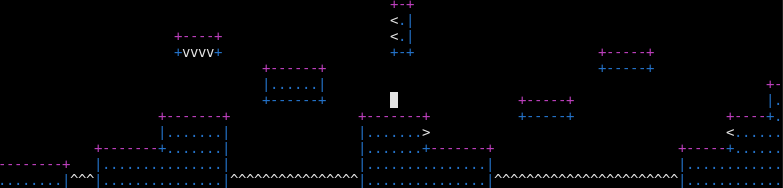
\includegraphics[width = 0.80 \textwidth]{content/affichage1.png}
		\end{center}
		
		Pour implémenter cette caméra, nous avons crée une structure caméra contenant :
		\begin{itemize}
			\item Des coordonnées centrales (x et y)
			\item Une longueur et une largeur \\
		\end{itemize}
		
		
		Ainsi, on repère la caméra selon son centre.
		\begin{center}
			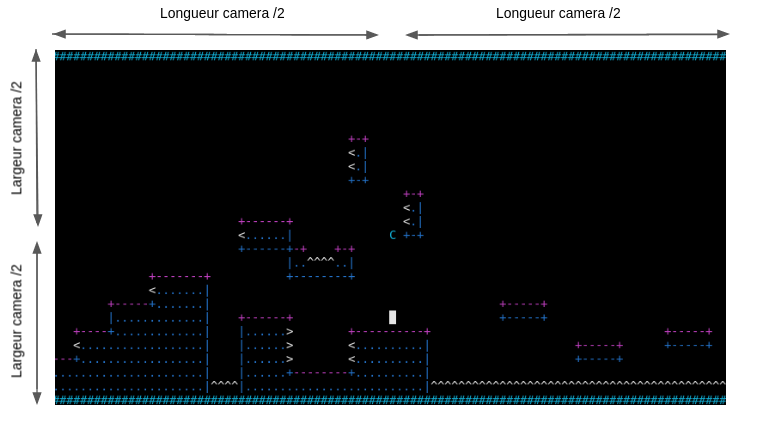
\includegraphics[width = 0.70 \textwidth]{content/affichage2.png}
		\end{center}
		
		Une caméra centrée apporte cependant un problème lorsqu'on approche des bordures de la carte.
		En effet, si le joueur est au bord de la carte, la caméra se devra d'afficher une partie de l'environnement qui n'existe pas. \\
		
		
		Pour pallier a ce problème, il existe plusieurs solutions dont le plus connu était :
		\begin{itemize}
			\item De bloquer la caméra à une certaine position
			\item D'afficher du vide
			\item De créer des bordures de map plus larges \\
		\end{itemize}
		
		
		Pour Platformer, nous avons choisi la première option.
		
		Ainsi, à partir d'une certaine position du joueur dans la carte, la caméra se bloque.
		Cette limite, que ne peut dépasser la caméra, est différente selon les deux axes x et y.
		\begin{center}
			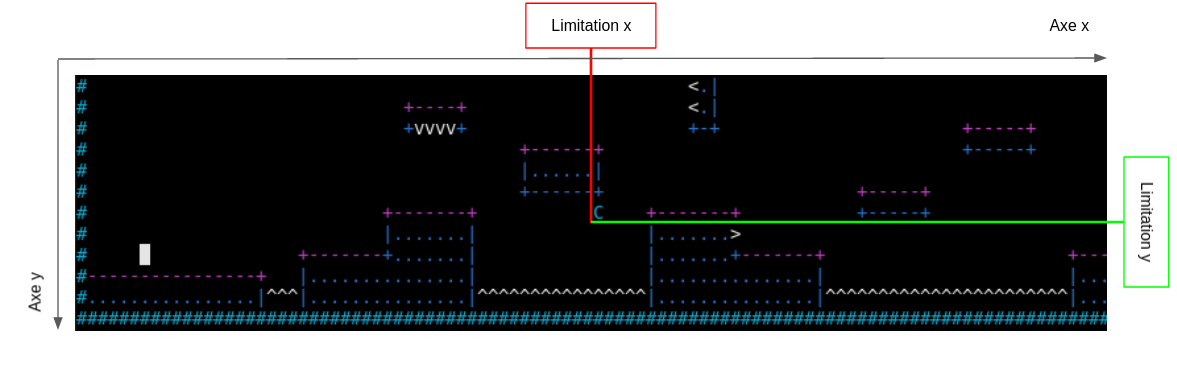
\includegraphics[width = 0.90 \textwidth]{content/affichage3.png}
		\end{center}
		
		Enfin, dans le cadre de Platformer, il faut prendre en compte un autre paramètre : la taille du terminal.
		En effet, il faut pouvoir définir la taille de la caméra en prenant en compte la taille de la carte mais aussi celle du terminal :
		Une carte plus petite que le terminal doit pouvoir être affichée en entière. \\
		
		
		Pour cela, on définit la caméra de même taille que le terminal, mais lorsque la taille devient supérieure à celle de la carte,
		alors on définit la caméra selon la taille de la carte. \\
		
		
		Ainsi donc, nous avons placé la limite, précédemment vus, dynamiquement par rapport à la taille du terminal : 
		Si le joueur se situe dans une partie de la carte dont la taille est inférieure à la moitié de la taille du terminal,
		alors la caméra se bloque contre cette limite. \\
		
		
		Tous ces choix nous ont permis d'avoir un affichage dynamique aussi bien par rapport à la taille du terminal que par rapport à la carte.
		\newpage

		\subsection{Collisions}
		
		Les collisions ont également été un point à la fois déterminant et complexe pour rendre le jeu fonctionnel. En effet, une partie de la complexité vient du fait que lorsque le personnage se tient près d'un mur, il doit ne plus pouvoir bouger s'il va dans la direction du mur, mais doit quand même pouvoir s'en éloigner.
		
		Ici encore, comme dans la physique, on a séparé les collisions sur \(x\) et \(y\), qui a un inconvénient, de mal pouvoir détecter les collisions en diagonales, mais qui reste quand même très rare à obtenir.
		
		La détection des collisions se fait de manière ordonnée (similaire pour l'axe \(x\) et \(y\)):
		\begin{enumerate}
			\item Dans un premier temps, on cherche dans quel sens va le joueur. On crée une variable \textit{sens} qui stocke ce sens. On se sert de la variable \textit{deltaPosition} pour le déterminer (cette variable est évoquée dans la partie "physique"). La variable sens peut prendre 3 valeurs : 
			\begin{itemize}
				\item -1 si le joueur va vers le bas sur \(Y\) (ou vers la gauche sur \(X\))
				\item 0 si le joueur est immobile sur l'axe en question
				\item 1 si le joueur va vers le haut sur \(Y\) (ou vers la droite sur \(X\))
			\end{itemize} 
			\item On vérifie que le joueur n'est pas en bord de carte (mais en incluant le sens sinon le joueur resterait collé à une paroi\dots invisible).
			\item Enfin, on stocke les caractères à droite et à gauche du joueur (qui ne peuvent pas dépasser les limites de la carte, car l'étape d'au dessus enlève ces cas particuliers).
			\item On vérifie ensuite qu'il n'y a rien dans la direction ou va le joueur. S'il n'y a rien, on renvoie \textit{false}, pour signaler qu'il n'y a aucune collision.
			Sinon, on sépare trois cas :
			\begin{itemize}
				\item Le premier, sur l'axe des \(X\) : ici, on enlève la vitesse sur \(X\) en mettant la valeur à 0 et on fait de même pour l'accélération
				\item Pour les \(Y\), si l'on touche quelque chose vers le bas : on fait pareil que sur les \(X\).
				\item Si le joueur touche quelque chose sur le haut, on remet la valeur de la vitesse à 0, met on celle de l'accélération à \(-g\) : le joueur est supposé dans le vide, donc subit toujours l'attraction "terrestre". Ce cas est le même dans le cas où le sens est nul (c'est à dire que le joueur est immobile sur les \(X\)) et qu'il n'y a rien en-dessous du joueur.
			\end{itemize}
		\end{enumerate}
	
		Une fois ces étapes exécutées, on obtient \textit{true} ou  \textit{false} selon si il y a collision ou non. S'il y a collision, alors la position du joueur n'est pas mise à jour (le joueur reste donc immobile).
		
		La vérification de la mort du joueur est également faite ici : puisqu'il n'y a pas d'ennemi, la seule façon de perdre est de tomber dans un trou ou de rentrer dans un pic. Pour vérifier, on regarde juste le caractère qui est après le joueur dans la direction où il va : si c'est un pic, on déclenche l'arrêt du jeu ; sinon on continue.
		
		
		
	\newpage

	\section{Conclusion}

	Parmi les idées qui auraient pû améliorer le jeu, nous avons retenu :
	\begin{itemize}
		\item Un menu pour choisir différentes cartes
		\item Des adversaires automatiques
		\item Des checkpoints
		\item Éventuellement, un outil pour créer d'autres cartes (ou un guide)
		\item \dots
	\end{itemize}
		
\end{document}